%When this chapter was first started in early 2022 `Web3' was at the peak of it's hype. Web3 is still a rapidly evolving set of technologies and specifications, which are drifting further from their origin. Decentralised web is perhaps a more useful name.%, but focus in this section will be on the evolution of the popularised term Web3. 
\section{Semantic web}
The ``semantic web'' definition of Web3.0 has been somewhat overhauled by other innovations in decentralised internet technologies, now evolving toward the slightly different Web3 moniker. Tim Berners Lee (of WWW fame) first mentioned the semantic web in 1999 \cite{semanticWeb}.\par
``I have a dream for the Web [in which computers] become capable of analyzing all the data on the Web – the content, links, and transactions between people and computers. A "Semantic Web", which makes this possible, has yet to emerge, but when it does, the day-to-day mechanisms of trade, bureaucracy and our daily lives will be handled by machines talking to machines. The "intelligent agents" people have touted for ages will finally materialize.''\par
Attention developed around three core themes, ubiquitous availability and searchability of data, intelligent search assistants, and highly available end points such as phones, and `internet of things' devices. This is certainly manifesting in home devices, but few people think of this as a Web3 revolution. 
\begin{comment}
The framework can be seen in Figure \ref{fig:semanticWebStack}.\par
\begin{figure}
  \centering
    \includegraphics[width=\linewidth]{semanticWebStack}
  \caption{\href{https://en.wikipedia.org/wiki/Semantic_Web_Stack}{Semantic Web Stack} [CC0 image]}
  \label{fig:semanticWebStack}
\end{figure}
\end{comment}
Since ratification of the standards by the \href{https://www.w3.org/standards/semanticweb/}{World Wide Web (W3C) consortium} it seems that their imperative toward decentralisation has become lost. Instead, it can be seen that Facebook, Amazon, Google, and Apple have a harmful oligopoly on users data \cite{costigan2018world}. This is at odds with Berners-Lee's vision, and he has recently \href{https://thenextweb.com/news/web-inventor-tim-berners-lee-screw-web3-my-decentralized-internet-doesnt-need-blockchain/}{spoken out about this discrepancy}, and attempted to \href{https://www.cnbc.com/2022/11/04/web-inventor-tim-berners-lee-wants-us-to-ignore-web3.html}{refocus the media} onto Web3.0. \par
It is worth taking a look at his software implementation called \href{https://solidproject.org}{Solid}, which is far more mindful of the sovereignty of user data.\par
``Solid is an exciting new project led by Prof. Tim Berners-Lee, inventor of the World Wide Web, taking place at MIT. The project aims to radically change the way Web applications work today, resulting in true data ownership as well as improved privacy. Solid (derived from "social linked data") is a proposed set of conventions and tools for building decentralized social applications based on Linked Data principles. Solid is modular and extensible and it relies as much as possible on existing W3C standards and protocols.'' \par
Excitement around this kind of differentiated trust model, hinted at in ubiquitous availability of data (and implemented explicitly in Solid), has led to exploration of different paths by cryptographers, and this will be described later. For instance, one of the main developers of Solid, \href{https://github.com/melvincarvalho/}{Carvelho}, is now a leading developer and propotent of Nostr, another very interesting option which will be described later. This technology space is prolific, but still comparatively young and small.\par
\section{Spatial web}
``The Spatial Web'', a blurring of the boundaries between digital and geospatial physical objects, seems to have developed from the strands in the original W3C scope around devices in the real world. It has been concentrating around AR and VR but is being marketed and amplified with the same references to availability of data (See Figure \ref{fig:deloitteSpatial} from a Deloitte accounting report). This too is finding little traction in practice, though obviously the component technologies continue to enjoy rapid development. Nonetheless, this interpretation of Web3 becomes valuable when examining Metaverse later.\par
\begin{figure}
  \centering
    \includegraphics[width=\linewidth]{deloitteweb3}
  \caption{\href{https://www2.deloitte.com/us/en/insights/topics/digital-transformation/web-3-0-technologies-in-business.html}{Deloitte Spatial Web Overview} Reused with permission.}
  \label{fig:deloitteSpatial}
\end{figure}
\section{Web3}
More recently Web3 is \href{https://trends.google.com/trends/explore?date=all&q=web3}{being touted} as a way to connect content creators directly to content consumers, without centralised companies acting as gatekeepers of the data. It implies that all users have a cryptographic key management system, to which they attach metadata, that they make requirements of peers with whom they communicate, and that they maintain trust `scores' with peers.\par
It seems likely that this new model is less driven by a market need, and more by the high availability of tools which allow this to happen (the ecosystems described later). Add to this a social response to the \href{https://finance.yahoo.com/news/meta-facebook-worst-company-of-the-year-yahoo-finance-165345819.html}{collapse in trust of companies such as Facebook} and other \href{https://reb00ted.org/tech/20220727-end-of-social-networking/}{social media platforms}\cite{torok2017cascading} (Figure \ref{fig:trustbarometer}). There is perhaps a wish by consumers to pass more of the economic incentive to content creators, without the `rent seeking' layer afforded by businesses, and a healthy dose of mania driven market speculation. \href{https://www.edelman.co.uk/sites/g/files/aatuss301/files/2022-01/2022\%20Edelman\%20Trust\%20Barometer_UK.pdf}{Edelman's latest trust report} is shocking, finding that trust in all institutions has slumped recently to all time lows, and their global survey found that: \textit{``Nearly 6 in 10 say their default tendency is to distrust something until they see evidence it is trustworthy. Another 64\% say it’s now to a point where people are incapable of having constructive and civil debates about issues they disagree on. When distrust is the default – we lack the ability to debate or collaborate.''}

\begin{figure}
  \centering
    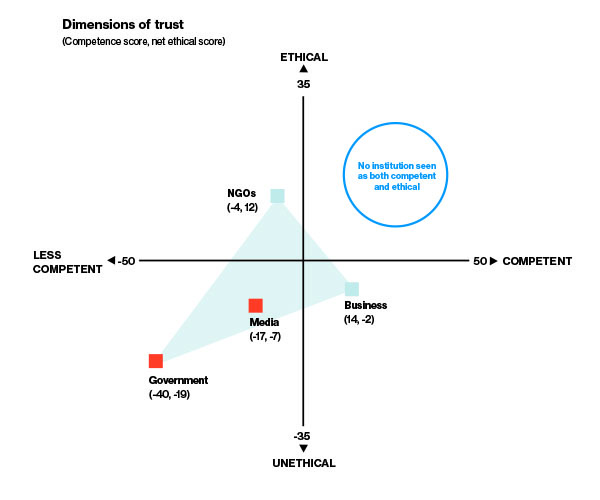
\includegraphics[width=\linewidth]{c-a-e}
  \caption{\href{https://www.edelman.com/trust/2020-trust-barometer}{Edelman 2020 trust barometer} [rights requested]}
  \label{fig:trustbarometer}
\end{figure}
\subsection{Emerging consensus}
The recent hype cycle ignored the legacy definitions described above and instead focusing almost exclusively on Ethereum based peer-to-peer projects. It can be seen that the description is somewhat in the eye of the beholder.\par
It's possible to frame this Ethereum Web3 as a hugely complex and inefficient digital rights management system (DRM). DRM is something that users of the internet are increasingly familiar and comfortable with. It's somewhat debatable whether decentralising this is worthwhile. The thesis of the developers of the technology seems to be that without it, control of `value' will accrete over time, to one or more hegemonic controlling entities. It's a strong argument, but there is a \href{https://moxie.org/2022/01/07/web3-first-impressions.html}{substantial counter argument} emerging that users just don't want this stuff. The nervousness of legislators in the USA to the attempt by Facebook/Meta to enter this peer-to-peer value transmission space is telling in terms of the perception of who is driving Web3.\par
Throughout 2022 there was much furore on the internet over what Web3 might be, and who it `serves'. Enthusiasts feel that products such as \href{https://blog.spruceid.com/sign-in-with-ethereum-is-a-game-changer-part-1/}{Sign-In with Ethereum} (EIP-4361) might give users choice over their data sovereignty, and a meme to this effect is seen in Figure \ref{fig:web1web2web3}. In practice though users are expecting to use badly written, buggy, economically vulnerable `crypto' wallets to log into websites. The quality of this wallet software is improving of late with the so called ``wallet wars'' seeing commerce grade offerings from Coinbase and shares platform `Robinhood'. These two companies alone have over 100 million users. It's likely that these wallets will evolve to offer the full spectrum of Web3 functionality. With that said it doesn't seem to make much sense yet on the face of it. There are in fact examples of the technology completely failing at censorship resistance. Popular `Web3' browser extension Metamask and NFT platform Opensea have both \href{https://www.forbes.com/sites/stevenehrlich/2022/03/03/iranian-venezuela-users-abruptly-dropped-from-major-crypto-platforms-as-russian-sanctions-grow/?sh=22bcabc470b0}{recently banned countries} in response to global sanction pressure. This failure to meaningfully decentralise will be explored further in the distributed identity section. \par
\begin{figure}
  \centering
   \includegraphics[width=\linewidth]{web1web2web3}
 \caption{A meme showing differing approached to logging in on a website.}
 \label{fig:web1web2web3}
\end{figure}
Of their 2022 \href{https://research.ark-invest.com/thank-you-big-ideas-2022?submissionGuid=0937b1ae-9e11-4b46-ae03-6cd8d2f8301b}{`Big Ideas' report}, ARK investment LLC (who manage a \$50B tech investment) \href{https://www.ark-bigideas.com/2022/en/pages/download}{said the following} (Figure \ref{fig:ARKWeb3}), which connects some of the dots already mentioned, and leads us into the next section which is Blockchain and Bitcoin:\par
\textit{``While many (with heavily vested interests) want to define all things blockchain as web3 we believe that web3 is best understood as just 1 of 3 revolutions that the innovation of bitcoin has catalyzed.
\begin{itemize}
\item The Money Revolution
\item The Financial Revolution
\item The Internet Revolution''
\end{itemize}}
\begin{figure}
  \centering
    \includegraphics[width=\linewidth]{Web3ARK}
  \caption{\href{https://twitter.com/wintonARK/status/1486143239753060353}{ARK slide on Web3.} Rights requested}
  \label{fig:ARKWeb3}
\end{figure}
This new hyped push for Web3 is being driven by enormous venture capital investment. A16Z are a \href{https://a16z.com/2022/01/07/9b-to-build-the-future/}{major player} in this new landscape and have released their \href{https://a16z.com/2022/01/07/how-to-build-a-better-internet-10-principles-for-world-leaders-shaping-the-future-of-web3/}{ten principles} for emergent Web3. Note here that A16Z are (like so many others) probably a \href{https://twitter.com/coryklippsten/status/1592242420137148416}{house of cards}.
\begin{itemize}
\item Establish a clear vision to foster decentralized digital infrastructure
\item Embrace multi-stakeholder approaches to governance and regulation
\item Create targeted, risk-calibrated oversight regimes for different web3 activities
\item Foster innovation with composability, open source code, and the power of open communities
\item Broaden access to the economic benefits of the innovation economy
\item Unlock the potential of DAOs
\item Deploy web3 to further sustainability goals
\item Embrace the role of well-regulated stablecoins in financial inclusion and innovation
\item Collaborate with other nations to harmonize standards and regulatory frameworks
\item Provide clear, fair tax rules for the reporting of digital assets, and leverage technical solutions for tax compliance
\end{itemize}
This list seems targeted toward the coming regulatory landscape, and could be considered at odds with the original tenants of an organically emergent, decentralised internet. Indeed principles such as `furthering sustainability goals' seem downright incongruous. The community they claim to wish to support here are openly critical of these major institutional players and their motives, with even more pointed criticisms \href{https://www.profgalloway.com/web3/}{coming from outside of the Web3}. This book and lab steer well clear of these companies and their applications.\par
Dante Disparte, chief strategy officer of `Circle' venture capital, said in testimony to a US senate hearing; that Web 1 was `read', Web 2 was `read write', and that Web 3 will `read write own'. The important takeaway here is not so much this oft quoted elevator pitch for Web3, but the fact that legislative bodies now consider this technology a force which they need to be aware of and \href{https://a16z.com/2021/12/17/prediction-for-the-new-year-a-web3-midterm/}{potentially contend with}.\par
Jeremy Allaire, again of Circle', talks about the recent legislative order in the USA as follows:
\textit{``this is a watershed moment for crypto, digital assets, and Web 3, akin to the 1996/1997 whole of government wakeup to the commercial internet. The U.S. seems to be taking on the reality that digital assets represent one of the most significant technologies and infrastructures for the 21st century; it's rewarding to see this from the WH after so many of us have been making the case for 9+ years.''}\par
We will see in the following chapters that participation in this new Web3 is contingent on owning cryptocurrencies. \href{https://www.finder.com/uk/cryptocurrency-statistics}{It's estimated} that about 6\% of people in the UK own some cryptocurrency, with skews to both younger demographics, and smaller holdings. The legislative landscape in the UK is comparatively strict with \href{https://uk.news.yahoo.com/perverse-impacts-anti-money-laundering-144239343.html}{questionable} ``know your customer / anti money laundering'' (KYC/AML) data collection \href{https://www.gov.uk/guidance/money-laundering-regulations-your-responsibilities}{mandated in law}. Users of UK exchanges must provide a great deal of personal financial information, and undertake to prove that the wallets they are withdrawing to are their own. From the perspective of the UK SME it seems this seriously limits the potential audience for new products. Europe meanwhile has recently voted through even more restrictive regulation, applying the ``\href{https://www.europarl.europa.eu/legislative-train/theme-an-economy-that-works-for-people/file-revision-of-the-regulation-on-transfers-of-funds}{transfer of funds regulation}'' to all transactions coming out of exchanges, enforcing a database of all addresses between companies, and reporting transactions above 1000 Euros to authorities. They have narrowly avoided enforcing KYC on all transfers to private wallets, but have capped transactions at 1000 Euros. The \href{https://www.consilium.europa.eu/en/press/press-releases/2022/06/30/digital-finance-agreement-reached-on-european-crypto-assets-regulation-mica/}{``Markets in Crypto Assets (MiCA)} legislation is an onerous overhead that will likely make it impossible for smaller businesses in the sector to operate within the EU. This is still short of the ban that they have \href{https://netzpolitik.org/2022/climate-measures-behind-closed-doors-eu-officials-talk-about-banning-bitcoin/}{discussed in private}. It seems that this EU position has prompted the UK government to seize the potential competitive advantage offered, and there will be more on this later. Japan meanwhile has gone so far as to \href{https://cointelegraph.com/news/japanese-prime-minister-says-gov-t-investment-in-digital-transformation-will-include-metaverse-nfts}{make an announcement} about supporting the technologies at a national level.\par
%Many of the mentioned components here will be described later in the book. The suggestion is that this is happening regardless of a decent use case or definition.\par
It's a complex evolving narrative, and clearly contradictions are common. Right now there seems little appeal for stepping into Web3. Into the confusion, this book advances a narrow take, and toolset, which might extract some value from the technologies, while maintaining a low barrier to entry.\par 
\begin{comment}
\section{Example applications}
It's handy here to get a feel for what this looks like. These aren't things that this book wishes to contribute to, or even have a firm opinion on, they're just representative of current activity in the decentralised web space.
\subsection{Podcasting2.0}
\href{https://medium.com/@everywheretrip/an-introduction-to-podcasting-2-0-3c4f61ea17f4}{Podcasting 2.0} leverages \href{https://www.rssboard.org/rss-specification}{RSS} (the original dissemination system for podcasts) and the Bitcoin Lightning network, to enable so-called `\href{https://www.youtube.com/watch?v=NO1aDZ6L4NQ&t=1123s}{value for value}' broadcasting. Subscribers use one of a variety of apps to stream micro-transactions of Bitcoin directly to the content creators as they listen to the podcast. No intermediate business takes a cut. Some variation on this model exists, such as John Carvalho's crowd funded podcast ``The Biz'' which progressively unlocks more minutes for everyone based on \href{https://thebiz.pro/about#crowdwall}{crowd funded donations}.
\subsection{Crowd funding}
At time of writing a \href{https://www.constitutiondao.com/}{crowd funding initiative} based around a digital decentralised construct called a DAO (explained later in detail) \href{https://www.coindesk.com/business/2021/12/06/daos-and-the-next-crowdfunding-gold-rush/}{managed to raise \$46 million dollars to bid for a copy of the US constitution} at Southerbys auction house. The attempt narrowly failed, but the press \href{https://www.coindesk.com/business/2021/12/09/what-kickstarter-going-decentralized-means-for-web-3/}{heralded this new era of ``Web3'' economic might}. This model might be the only use for DAOs and is likely just a way to avoid regulatory scrutiny. There is more detail on DAOs later.
\subsection{Distributed exchanges}
There are dozens of decentralised exchanges deployed on various blockchains. These platforms allow users to trade back and forth between various tokens (including `normal money' stablecoins) and charge a fee for doing so. They operate within the logic of the smart contracts \cite{szabo1997formalizing}, within the distributed blockchains. This makes them extremely hard to ban, and as a result they operate in a legal grey area. At the extreme end of this is ``distributed apps'' (dApps) and ``Decentralised Finance'' (DeFi) which allows users access to complex financial instruments without legal or privacy constraints. DeFi will be touched on briefly later.\par
This is a huge area, and of only limited interest to the topics expanded in this book. It's perhaps worth noting \href{https://bitcoin-dex.net/about/index.html}{BitcoinDEX}, which runs in JavaScript in a web browser. It is effectively uncensorable, \href{https://bitcoin-dex.net/tokens.js}{auditable by the user}, and has no counter party risk since it operates entirely in the Bitcoin network. It is clearly an early prototype but manages this complex feature without the more expressive logic of more `modern' public blockchains.
\subsection{NFT marketplaces}
NFT markets are far more centralised services which match `owners' of digital assets with potential buyers. The concept is a staple of the more recent interpretation of Web3, even though in practice these seem to be centralised concerns. \href{https://opensea.io/}{Opensea} claims to be the largest decentralised NFT marketplace, but they have the ability to \href{https://thedefiant.io/sad-frogs-delisted-opensea/}{remove listings} in response to legal challenges. This seems to fly in the face of Web3 principles. NFTs are currently a \href{https://tante.cc/2021/12/17/the-third-web/}{deeply flawed} technology but seem likely to persist and will be covered later.
\subsection{Non blockchain webs of trust}
New products like Slashtags and Nostr (covered later) use a web of trust decentralised peer-to-peer (ish) model which assigns metadata and trust scores to `any' data and connection, with a security model rooted in the Bitcoin cryptographic `keys' but crucially not the bitcoin network. This makes it interoperable with bitcoin but not reliant upon it. In principle this allows users to build complex networks of inherited trust bi-directionally with their networks over time. Every connection to a peer can be a new schema, with individual metadata managed by the user. These are new and have low adoption at this time. The user controls the source of the data and can allow them to be used by centralised services. This flips the authentication and data management paradigm of web around, putting the user in charge of their data. This is a familiar concept to the DID/SSI communities (described later) but with significant investment. As Slashtags and Nostr use keys as endpoints they act as a web of naming and routing, bypassing the existing web infrastructure of DNS. It is likely very complex to use in practice and will be revisited later. Slashtags is being paired with the \href{https://hypercore-protocol.org/}{Hypercore protocol} for peer-to-peer data sharing, more specifically the `hole punching' capability of the hypercore system which ensures connections through firewalls\cite{ford2005peer}. The first application by the affiliated Hyperdivision team is an open source peer-to-peer live video streaming app called \href{https://dazaar.com/}{Dazaar}. Once again, it's not clear yet who wants or needs this bit-torrent style service. 
\subsection{Distributed DNS applications} 
There are many perceived problems with having centralised authorities for overseeing the database which translates between human readable internet names and the underlying machine-readable address notation. The databases which manage this globally are already somewhat distributed, and this distributed trust model is managed through a cryptographic chain of trust called DNSSEC which is capped by a somewhat \href{https://www.iana.org/dnssec/ceremonies}{bizarre key ceremony} seen in Figure \ref{fig:dnssec}. The authority around naming is centralised in ICANN. 
\begin{figure}
  \centering
    \includegraphics[width=\linewidth]{dnssec}
  \caption{\href{https://www.internetsociety.org/blog/2016/10/watch-live-today-dnssec-root-ksk-ceremony-at-1700-utc/}{DNSSEC ceremony in a faraday cage}}
  \label{fig:dnssec}
\end{figure}
There has been talk for many years about `properly' distributing this database using decentralised/blockchain technologies\cite{karaarslan2018blockchain}. The nature of this problem means that it either moves from control by ICANN, or it does not, and so far it has not, but there are many attempted, and somewhat mature attempts, at this difficult problem. Of these \href{https://www.namecoin.org/}{Namecoin} is the most prominent, and is a fork of Bitcoin. The ubiquity of Bitcoin in such systems is perhaps becoming apparent.
\subsection{Impervious browser}
It might be that the future of Web3 comes in the guise of integrated suites such as the proposed \href{https://newsletter.impervious.ai/impervious-browser-functionality-overview/}{Impervious web browser}. They say that ``without centralized intermediaries'' it features:
\begin{itemize}
\item    Zoom, without Zoom.
\item    Google Docs, without Google.
\item    Medium, without Medium.
\item    WhatsApp, without WhatsApp.
\item    Payments, without banks.
\item    Identity, without the state.
\end{itemize}
This is obviously leading marketing hype, and they're already late for their release deadline, but what they're talking about here is an integration of the components mentioned in this book. If they can get critical mass around this browser then perhaps the Web3 market can be kickstarted. CEO Chase Perkins has \href{https://www.youtube.com/watch?v=2J8v-TMygK8}{recently presented} on this.
\end{comment}
\section{The common thread}
One feature which persists throughout all of these interpretations of Web3 is the need for decentralised trust. According to \href{https://www.coindesk.com/podcasts/the-breakdown-with-nlw/yesterdays-hearing-was-cryptos-most-positive-interaction-with-the-us-government-ever/}{Nathaniel Whittemore}, a journalist for Coindesk, ``The Web3 moniker positions this industry in opposition to big tech''. Alternatively the \href{https://cryptocriticscorner.com/}{many detractors} of the technology think it simply provides avenues for incumbents to experiment with new \href{https://www.cigionline.org/articles/amid-the-hype-over-web3-informed-skepticism-is-critical/}{models of control and monetisation}, \href{https://newsletters.theatlantic.com/galaxy-brain/624cb2ebdc551a00208c1524/crypto-bubble-web3-decentralized-finance/}{increasing systemic risk} at no cost to themselves.\par %as in \href{https://stripe.com/gb/use-cases/crypto}{this announcement} from Stripe, the worlds biggest payment processor. 
Overall then, perhaps the space is hype, and is certainly \href{https://web3isgoinggreat.com/}{rife with scams}. Fully 24\% of projects in 2022 are \href{https://blog.chainalysis.com/reports/2022-crypto-pump-and-dump-schemes/}{estimated to be built} as `pump and dump' scams. The degree to which it even accomplishes decentralised trust is highly debatable, and meanwhile the limited numbers of Web3 and supporting crypto companies display lamentable cyber security practice themselves, creating \href{https://www.coindesk.com/tag/data-breaches/}{honeypots of personal data} from users of the ecosystem.\par
With that said the component parts necessary to deliver on the promise \textbf{do} exist. If there is to be no central controlling party(s) as in the Web 2 model then nothing can happen without a cryptographically secure underpinning, allowing digital data to be passed around without a prior arrangement.\par%which favours no party beyond the terms of their collectively agreed rights and privileges. 
The following chapter will describe how much has been done by computer scientists over the past decades to support that. From this base layer we also get the potential for secure and trust minimised identity management. This nascent field of distributed identity management is explained later. From distributed trust models we can see `trustless' transmission of economic value. The ability to send value from one person to another person or service without a third party. \par
This whole area is `crypto', which is increasingly seeping into the human consciousness, and saw an astonishing \$30B of \href{https://docsend.com/view/nrvsuae85a4dx3jz}{capital investment in 2021} alone. At time of writing the industry is an \href{https://www.coingecko.com/en}{over 1 trillion} dollar market. \par
All the new crypto technologies circling the Web3 narrative are bound tightly together, but there is currently very little meaningful value to be seen.\par
The rest of this book will focus on the trust and value transfer elements of this shift in internet technologies, and attempt to build a case for it's use in decentralised, open source, collaborative mixed reality applications.
%\section{Risks}
